\section{Our Approach}\label{sec:approach}

\begin{figure}
  \centering
  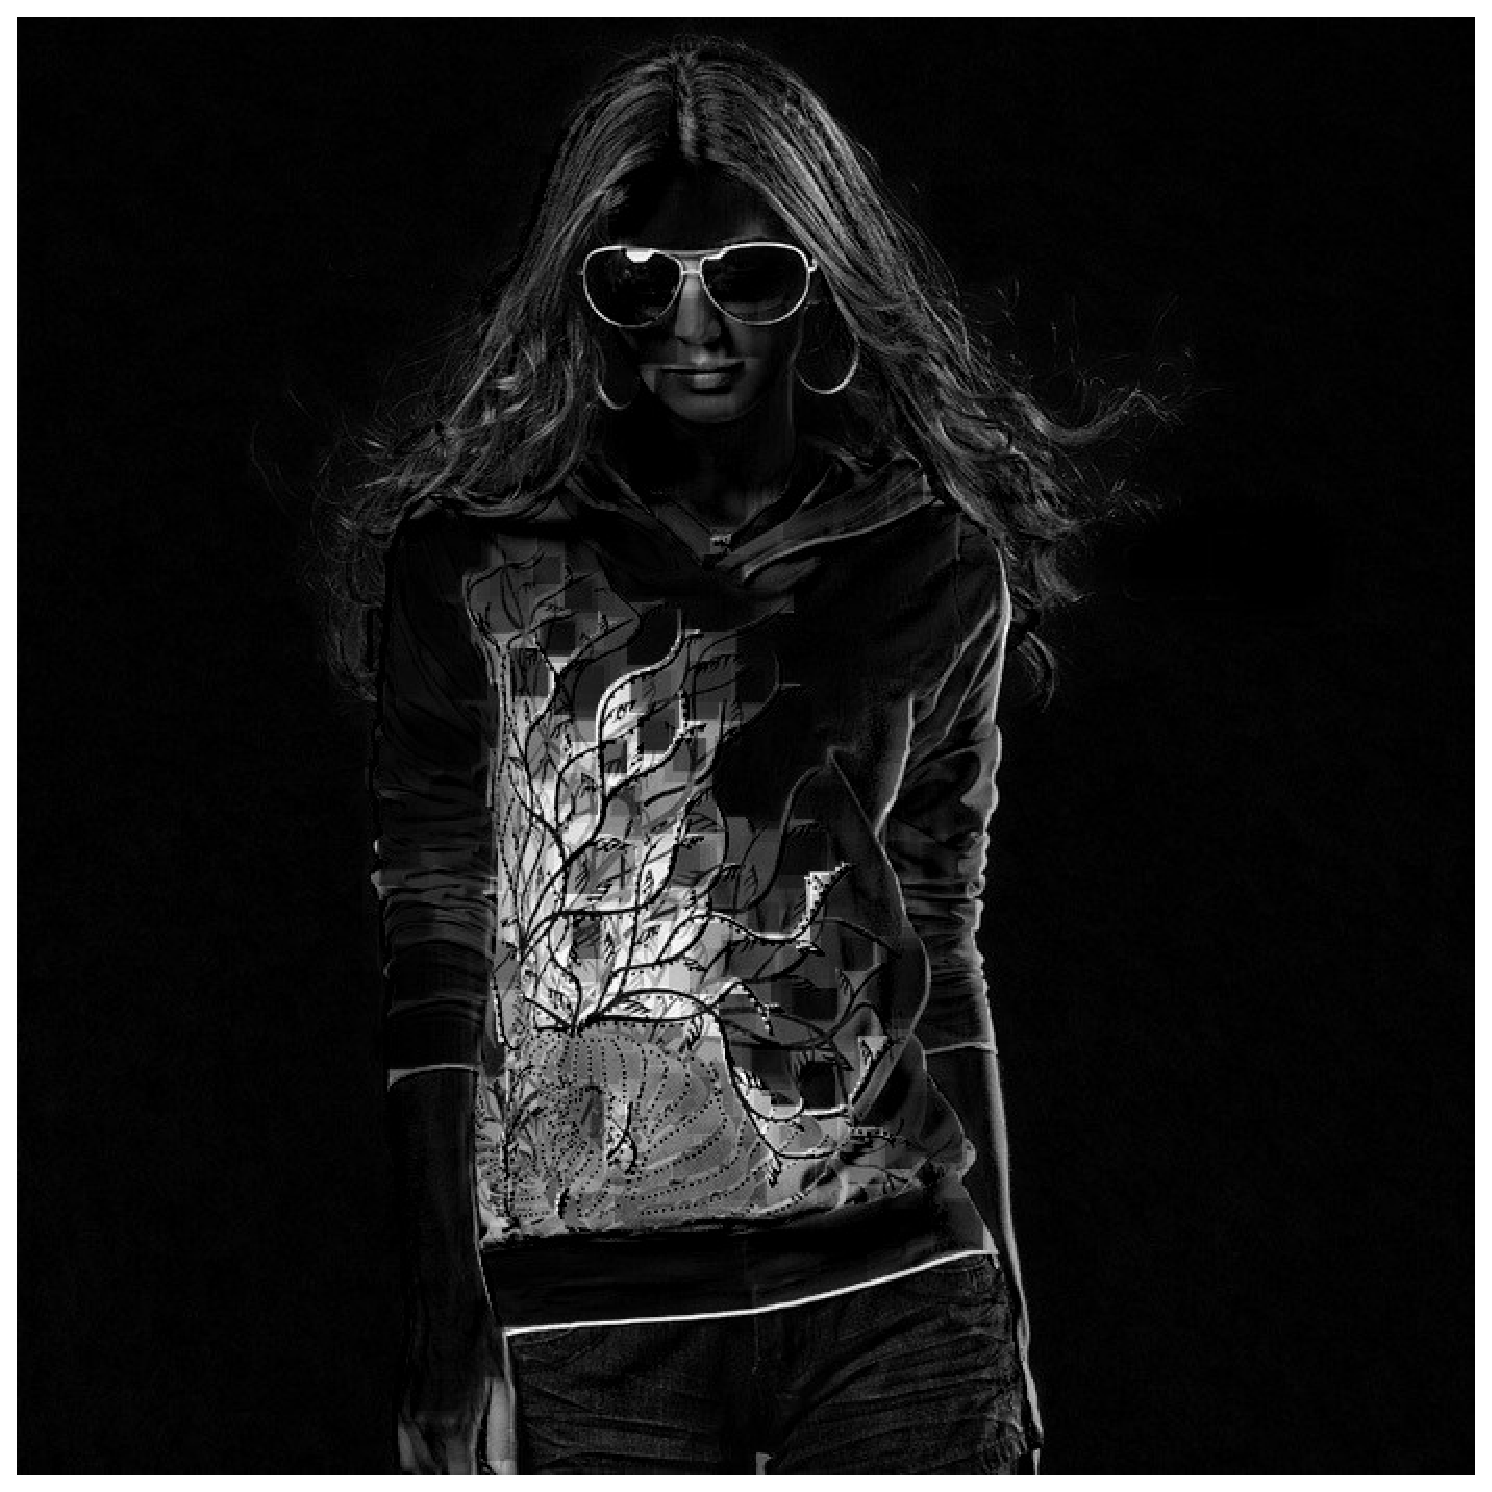
\includegraphics[width=0.7\textwidth]{image1}
  \caption{Image Preprocessing Example1}
  \label{fig:image1}
\end{figure}

\begin{figure}
  \centering
  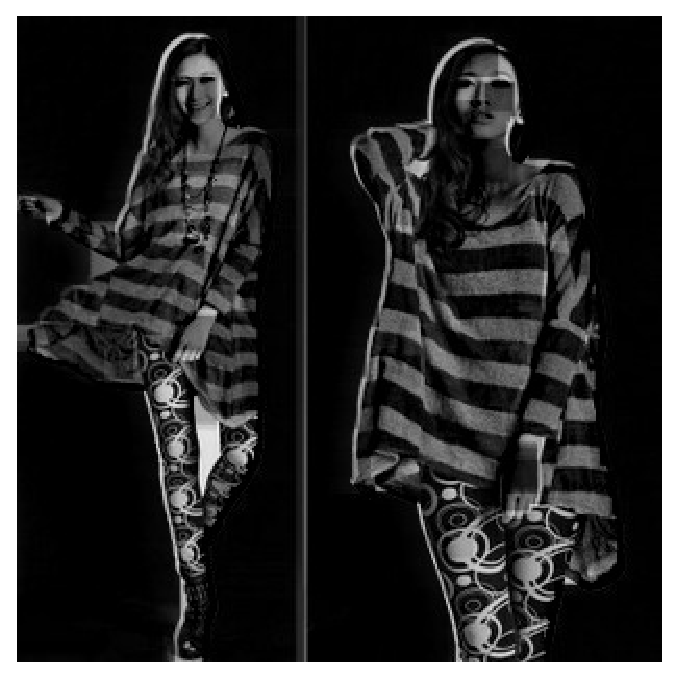
\includegraphics[width=0.5\textwidth]{image2}
  \caption{Image Preprocessing Example2}
  \label{fig:image2}
\end{figure}

\subsection{Model apparel item}
In this section, we will mainly talk about how to model the apparel item from two dimensions. One is the textual labels and the other is the images affiliated to the apparel. The vectors of them will be combined by weight to characterize the textual labels and the image feature of the apparel.

\subsubsection{Vectors of textual labels}
The first step is to process text labels. A certain number of keywords could be picked to describe clothing characteristics like \emph{long sleeve} in sleeve length, \emph{leisure} in styles and \emph{cotton} in fabrics. Then a vector in binary is used to record such features for both clustering and feature selection. If the apparel item contains that feature in its textual label, we can mark 1 in the corresponding place of the textual vector. If not, mark 0.

\subsubsection{HAC textual labels}
In the next step, HAC (Hierarchical Agglomerative Clustering) was employed to reveal similarities among the text labels of different 
garments, then we manually set a threshold as the number of clusters to divide all the garments to several groups, which serve as the basis for future classification.
In our approach HAC is preferred because it could produce an ordering of the objects, which may be informative for future classification.  In addition, multiple measures of distance can be used, however for simplicity we only focus on Euclidean distance and regard the mean distance between elements of each cluster as the distance between clusters.

\subsubsection{Preprocessing images}
For images, at first they are preprocessed to gray-scale pictures with minimum disturbance from the background and the photo model, which is approached by morphological manipulation using OpenCV. Figure \ref{fig:image1} and Figure \ref{fig:image2} shows two examples of the images after preprocessing by OpenCV. We can see from the images that the disturbance of the background is mostly eliminated. Thus the features we used to further represent the images are mainly the apparel information itself.

\subsubsection{Learn dictionary of images with K-SVD algorithm}
K-SVD \cite{ksvd}algorithm, which generalizing the K-Means clustering process, is for adapting dictionaries in order to achieve sparse signal representations. Using an overcomplete dictionary matrix $\mathbf{D \in \mathbb{R}^{n\times K} }$ that contains $\mathbf{K}$ atoms, $\{d_j\}_{j = 1}^K $ , as its columns, it is assumed that a signal $\mathbf{y \in \mathbb{R}^n}$ can be represented as a sparse linear combination of these atoms. The representation of $y$ may either be exact $\mathbf{y = Dx}$, or approximate, $\mathbf{y} \approx \mathbf{Dx}$, satisfying $\|\mathbf{y - Dx}\|_2 \leq \epsilon$. The vector $x \in \mathbb{R}^K$ displays the representation coefficients of the signal $\mathbf{y}$. This, sparsest representation, is the solution of either 
\begin{equation}
(P0 )\quad    min_x\|x0\|\quad subject\quad to \quad\mathbf{y = Dx}
\end{equation}
 or 
\begin{equation}
(P0, \epsilon)\quad    min_x\|x0\| \quad  subject\quad  to \quad \mathbf{\|y - Dx\|}_2 \leq \epsilon
\end{equation}
where $\|\cdot\|_0$ is the $l^0$ norm, counting the non zero entries of a vector.\\

The K-SVD is an algorithm designed to find the dictionary $\mathbf{D}$ that yields sparse representations for a set of training signals. A full description of the algorithm is given in Figure \ref{fig:ksvd}.\\
\begin{figure}
  \centering
  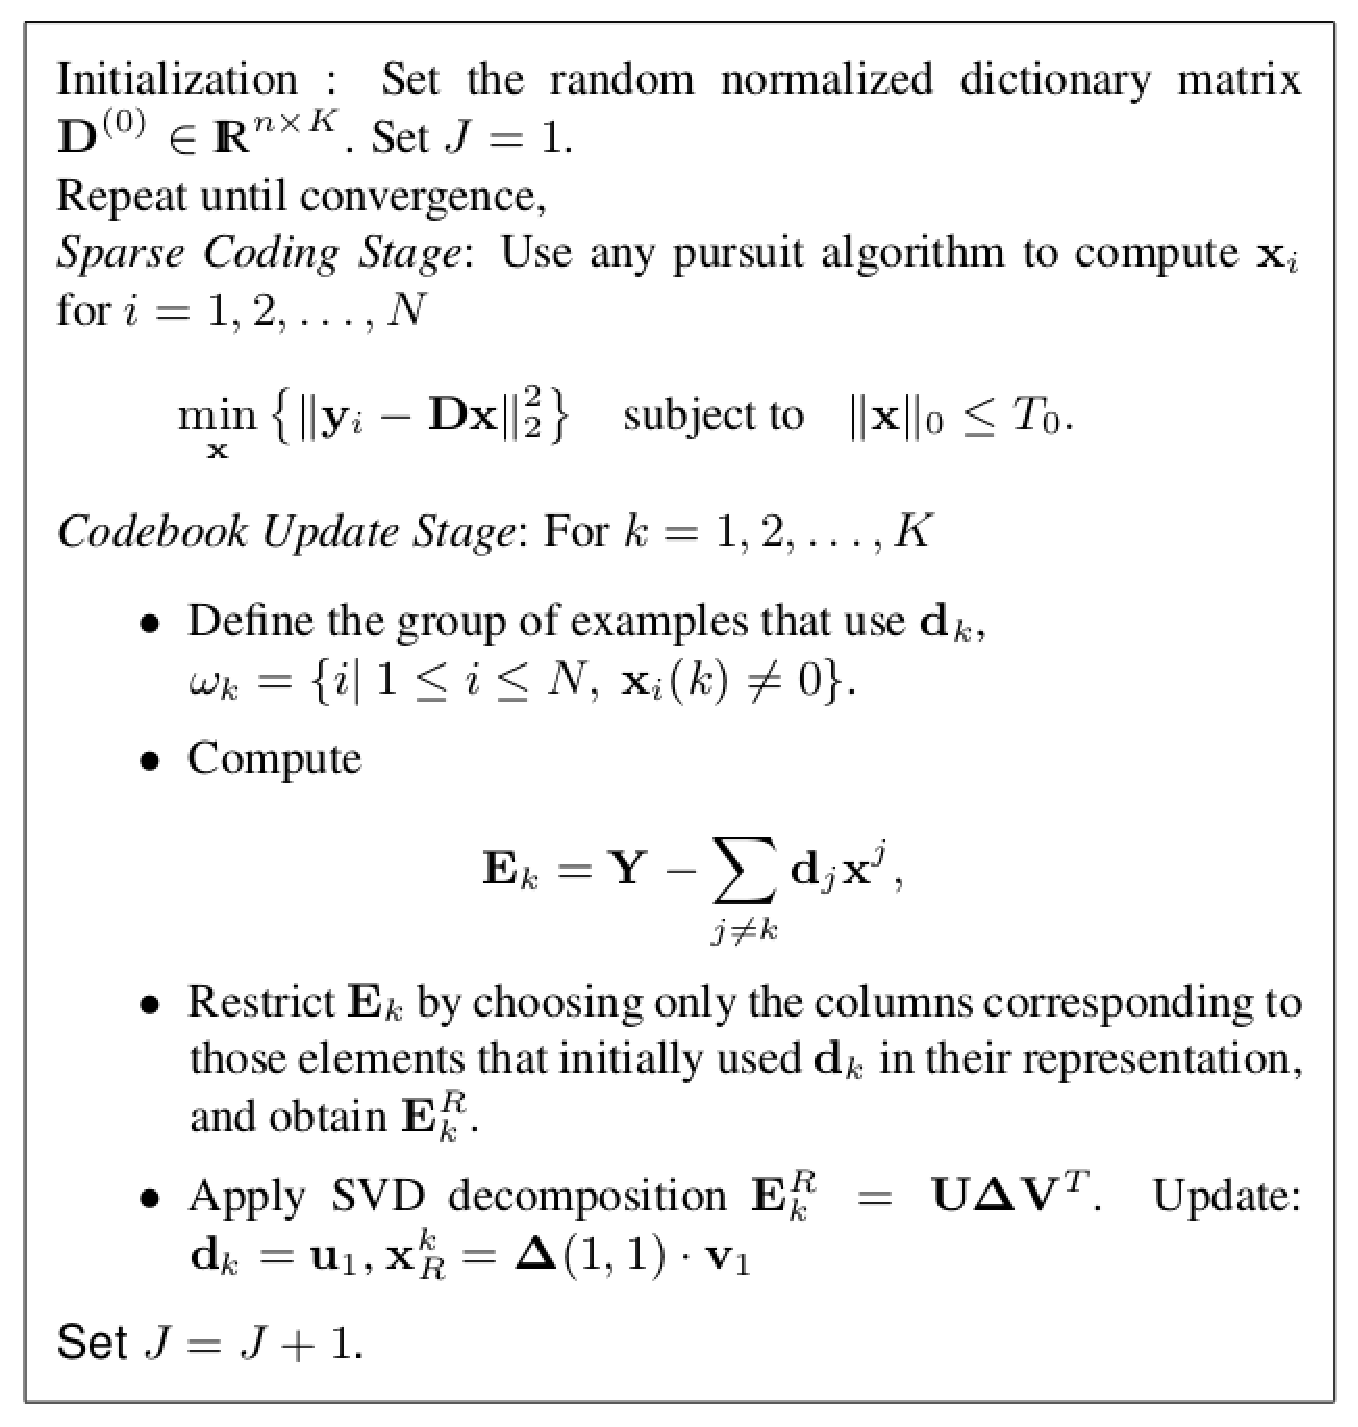
\includegraphics[width=0.5\textwidth]{KSVD}
  \caption{The K-SVD Algorithm}
  \label{fig:ksvd}
\end{figure}


We fisrt classified the whole apparel items into 30 classifications according to their similarity in the textual labels in HAC, which can enhance the accuracy of the learned dictionary as well as the recommendation. The classifed code wrote in Matlab is attached in our appendix. We will learn dictionary from each apparel set. Consequently we will get 30 dictionaries corresponding to each apparel set. After we applied the K-SVD algorithm to the apparel images, we get the trained dictionary like Figure \ref{fig:dict} shows. The dictory acts as the base vector of all the images for that apparel set.


\begin{figure}
  \centering
  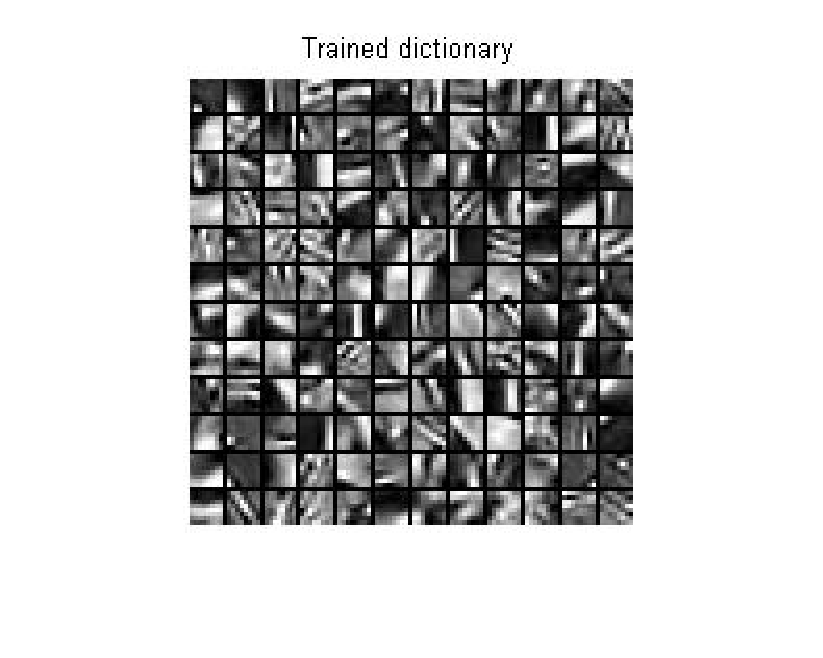
\includegraphics[width=0.5\textwidth]{Trained_dic}
  \caption{Dictionary Learned by K-SVD}
  \label{fig:dict}
\end{figure}


\subsubsection{Learn vectors of images}
Then sparse coding is applied with respect to the learnt dictionary to delineate pictures by feature vectors. The vectors are the representation coefficients of the input image signal. Thus each image can be successfully represented and be ready for machine learning. It is also noted that if a garment contains several pictures, it would be treated as several garments of the same text labels and scores.
  
\subsubsection{Comine vectors by weight}
And finally the binary vector constructed from text labels would be concatenated to another vector which describes image features to represent the whole features. These two features will be combined by a certain weight. This weight is varied from different people as the focus on textual labels or on apparel images is varied from person to person. In our framework, we have proposed a novel method that can effectively learn the weight for a specific user. We test the recommend accuracy for the user with different weight and choose the one that will result the best accuracy. In other words, the weight we choose can best fit the model of the user's inclination to textual labels an image features.

\subsection{Model user preference}
In this section, we will illustrate how to model the user preference and why we choose this way to model it.

\subsubsection{Get user preference and model it}
In our current way of collecting user preference, for every user, he or she will judge a garment based on personal preference with scores from 1 to 5. All the choices for clothing are recorded for future recommendation. Then based on the certain user's previous choices, the potential high-score garments can be predicted and thus being recommended. On the other hand, in real E-commerce systems, the preference can be collected through some records of user actions, including scanning time, favorite items, purcahse history or some clicking records, etc. These actions will be tracked by our framework and we use ratings to represent user preference. For instance, a user's favorite items would have a higher rating than other items who is not in his favorite items set but with the similar scanning time or clicking records. However, we are still on the way to quantify the exact rating from these actions. 
  
\subsubsection{Map apparel item to user preference}
Once we get the user's preferences (scores) on some garments, the relationships between these garments and their scores on this particular user have been established, which are serving as a training set.

\subsection{Recommend by rating}
In this section, how to recommend from the relationship of the apparel model and the user preference model will be covered. In our framework we leverageed the SVM algorithm to do the recommendition and we also proposeed another effective way to recommend.

\subsubsection{Support Vector Machine}
In machine learning, support vector machines (SVMs) are supervised learning models with associated learning algorithms that analyze data and recognize patterns, used for classification and regression analysis. The basic SVM takes a set of input data and predicts, for each given input, which of two possible classes forms the output, making it a non-probabilistic binary linear classifier. Given a set of training examples, each marked as belonging to one of two categories, an SVM training algorithm builds a model that assigns new examples into one category or the other. An SVM model is a representation of the examples as points in space, mapped so that the examples of the separate categories are divided by a clear gap that is as wide as possible. New examples are then mapped into that same space and predicted to belong to a category based on which side of the gap they fall on.
In addition to performing linear classification, SVMs can efficiently perform non-linear classification using what is called the kernel trick, implicitly mapping their inputs into high-dimensional feature spaces.

\subsubsection{Leverage SVM in our framework}
In our framwork, the inputs is the apprel set, the vectors combined by textual labels and image features, and the classes the apprel item is mapped is the corresponding preference ratings for an specific user.Then we use SVM to estimate the rating of other garments, based on which, we pick the highest ones to recommend. 
Note that this whole process is based on this particular user's preference. As is mentioned above, different users have different map according to their own model of user preference. 
As for the parameter selection for SVM, we applied grid search technique to find the optimal parameter set, i.e. we enumerate all the possible choices of parameters within a reasonable range and choose the one with the best cross-validation result and apply this parameter set for the future recommendation.

\subsubsection{Other options}
There's also another optional way to recommend. 
The garments we recommend will have a high possibility of user's preference, 
  which is derived from the relationship between the preference models of different users.

\subsection{Theoretical model}
Formally, suppose there are $K$ keywords in total, then every item $I$ has an associated 
  $K$-dimensional vector $T(I)$ where each dimension is either 0 or 1 which indicates the 
  existence of the corresponding keyword in the text labels of item $I$.
For an item $I$ and a user $U$, let $s(U,I)$ denote the score of $I$ given by $U$. 
Let $M(I)$ be the collection of all the images of $I$, $D$ be the learnt dictionary, and
  $C(M,D)$ be the sparse coding of $M$ using $D$.
Then the training set can be represented as $$ \{ [C(M^*,D), T(I), s(U,I)] : M^* \in M(I) \} .$$
